%***************************************************************************
\section{Propagation of the Prior Uncertainties}\label{sec:reflood_prior_uq}
%***************************************************************************

Hence, the \emph{prior uncertainty propagation} step constitutes of generating samples for each model parameter from its prior \gls[hyper=false]{pdf}, 
carrying out a set of \gls[hyper=false]{trace} simulations of the \gls[hyper=false]{feba} model using the sampled parameters, 
and analyzing the results to quantify the uncertainty of the model prediction.

\begin{sidewaysfigure}
	\centering
	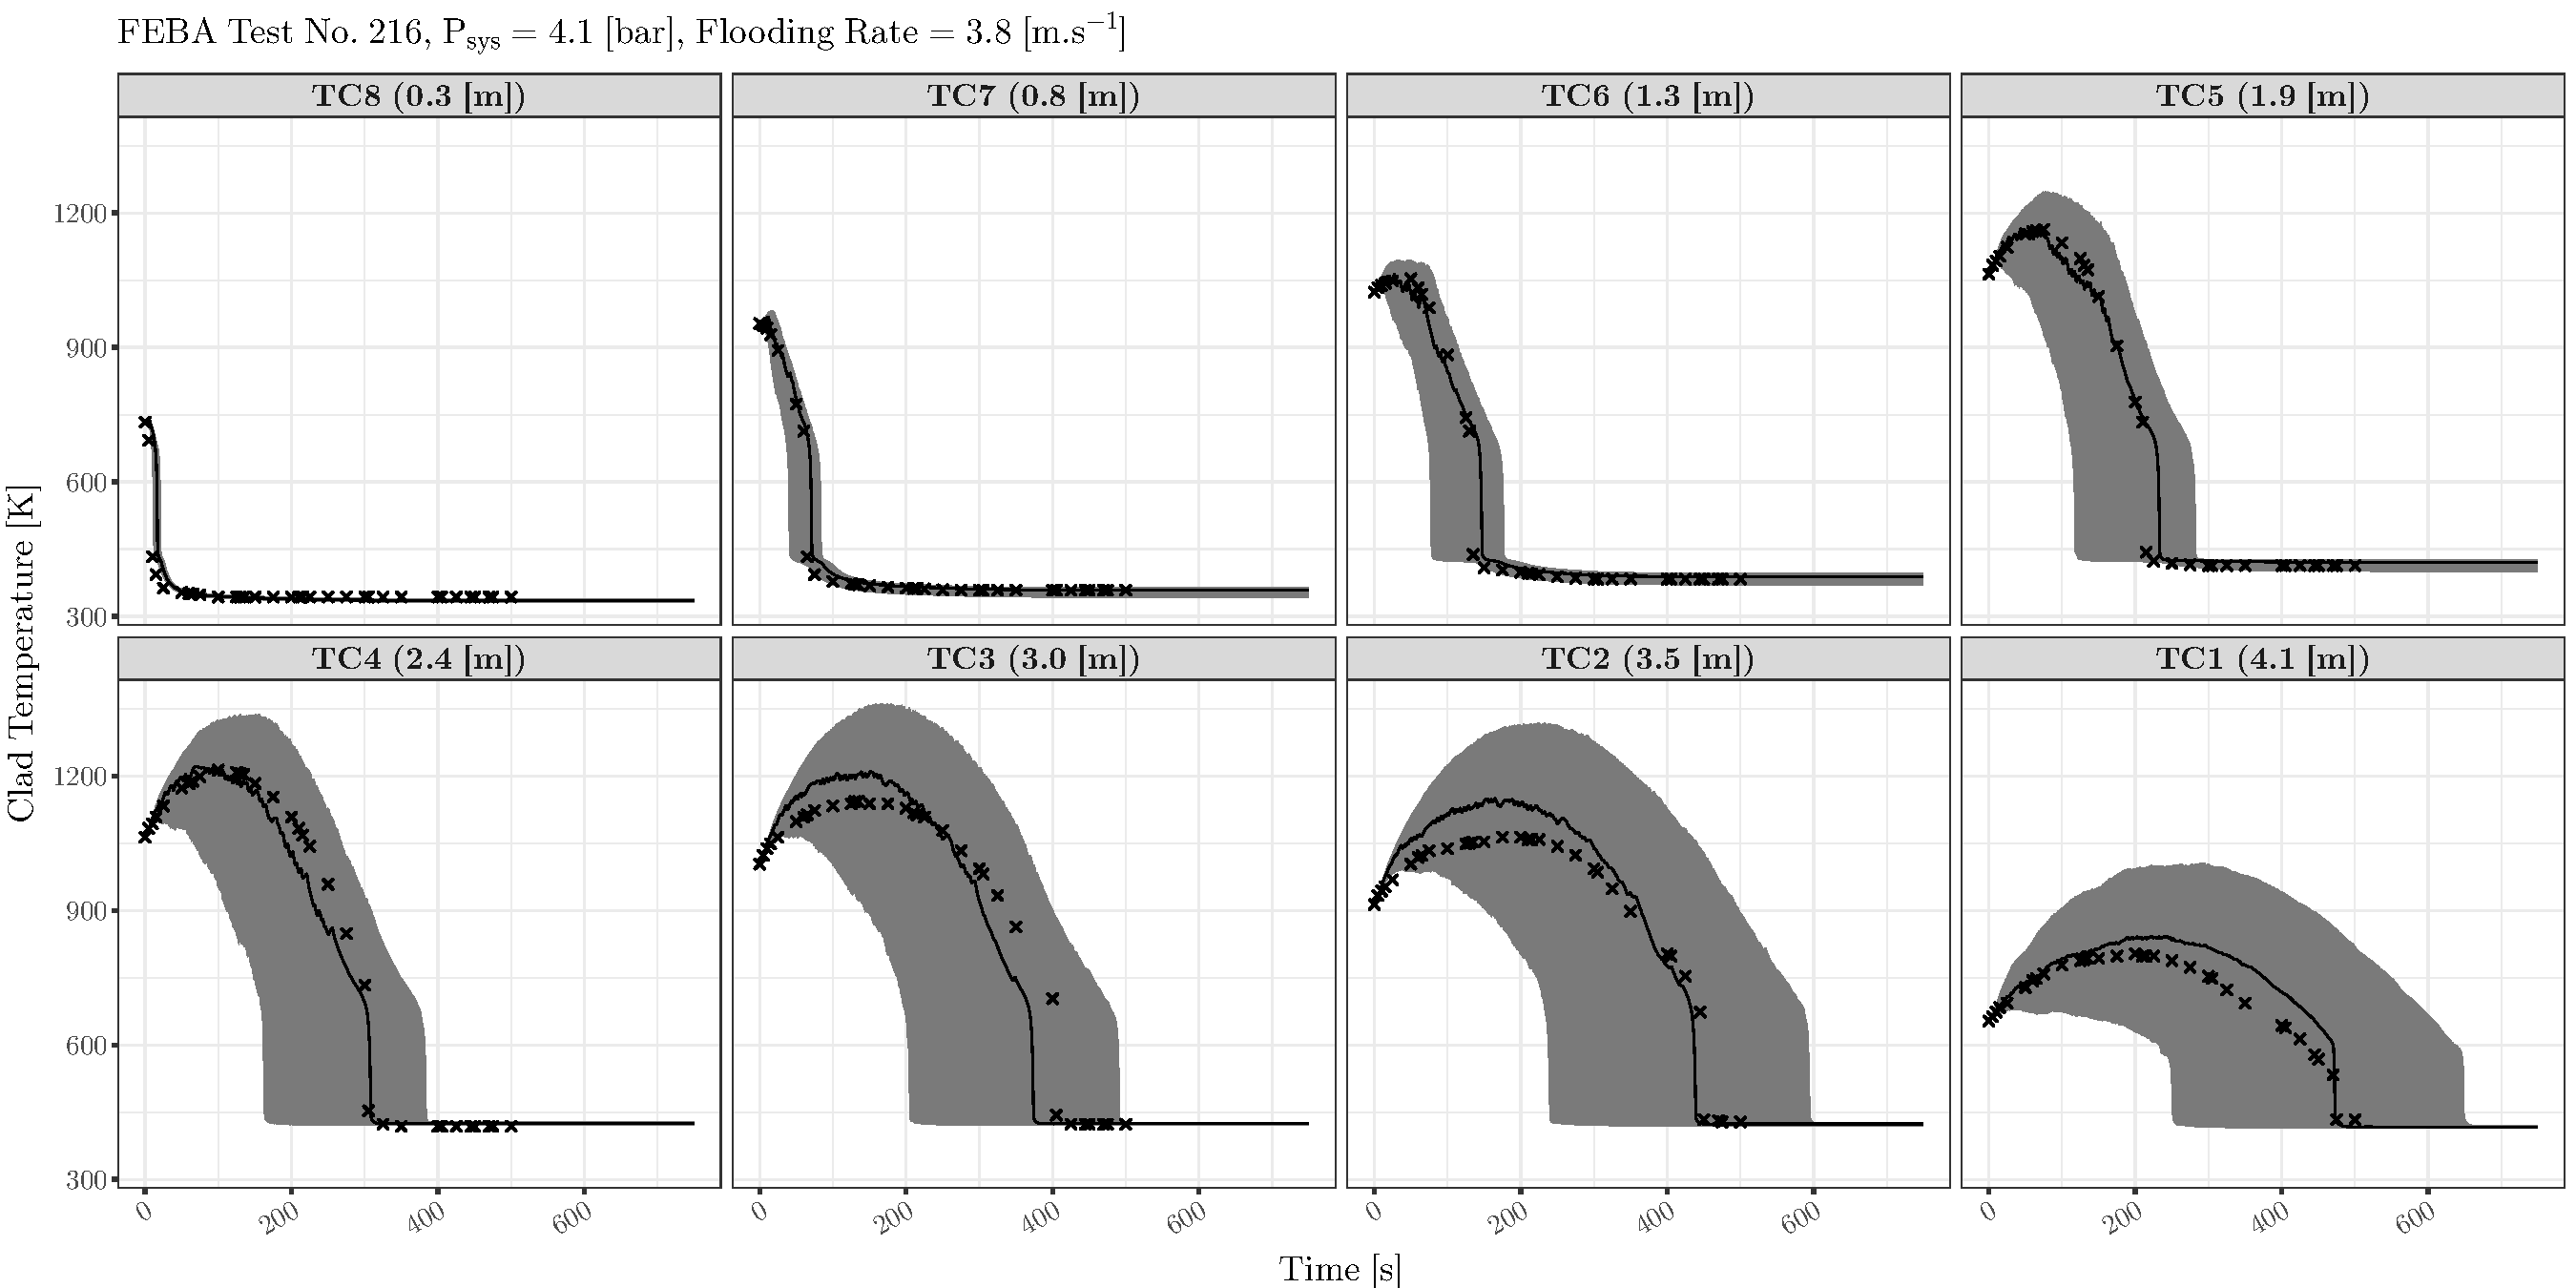
\includegraphics[width=0.90\textwidth]{../figures/chapter2/figures/plotTraceUQPriorTC216}
		\captionof{figure}[Propagation of the model parameters prior uncertainty on FEBA test No. $216$ for the cladding temperature output ($TC$)]{Propagation of the model parameters prior uncertainty on FEBA test No. $216$ for the cladding temperature output ($TC$) at different axial locations. The uncertainty bands refer to the symmetric $95\%$ probabilities. Solid lines, dashed lines, and crosses indicate the simulation with the nominal parameters values, the median of the posterior, and the experimental data, respectively.}
	\label{fig:ch2_plot_trace_uq_prior_tc_216}
\end{sidewaysfigure}
